\documentclass{article}
\usepackage[english]{babel}

\usepackage[a4paper,bottom=3cm,top=2.5cm,foot=1.5cm,left=1.75cm,right=1.75cm]{geometry}

\usepackage{fontspec}
\setmainfont[Mapping=tex-text]{LinLibertineO}
\newfontfamily\ipa{LinLibertineO}
\setsansfont[Scale=MatchLowercase]{Carlito}
\setmonofont[Scale=MatchLowercase]{DejaVu Sans Mono}

\usepackage{url}
\usepackage{graphicx}
\usepackage{longtable}

\usepackage{color}
\usepackage{colortbl}

\usepackage[table]{xcolor}
\usepackage{booktabs}

\usepackage{lastpage}
\usepackage{datetime}
\usepackage{textpos}
\usepackage{xltxtra}

\definecolor{gris}{rgb}{0.4,0.4,0.4}
\definecolor{morado}{cmyk}{0.09,1,0,0.3}
\definecolor{azul}{cmyk}{1,0.64,0,0.06}


\usepackage{fancyhdr}
\pagestyle{fancy}

% headers y footers
% borramos los estandares
\fancyhf{}
% y le sacamos esa horrible raya que viene por default
\renewcommand{\headrulewidth}{0pt}
\renewcommand{\footrulewidth}{0pt}

% numero de pagina
\fancyfoot[R]{\oldstylenums{\thepage}/\oldstylenums{\pageref{LastPage}}\quad\quad}

\usepackage{hyperref}
\hypersetup{pdftitle={Ramiro Vignolo--Curriculum Vitae}, pdfauthor={Ramiro Vignolo}, pdfkeywords={}, pdfborder={0 0 0}}

% background
\usepackage{eso-pic}
\newcommand\BackgroundPic{
\put(0,0){
\parbox[b][\paperheight]{\paperwidth}{%
\vfill
\centering

\includegraphics{logos/back.pdf}%
\vfill
}}}

% longitudes
\newlength{\chico}
\setlength{\chico}{0.5cm}

\newlength{\grande}
\setlength{\grande}{1.0cm}

\newlength{\ancholeft}
\setlength{\ancholeft}{1.7cm}
\newlength{\anchomain}
\setlength{\anchomain}{13.0cm}
\newlength{\anchoright}
\setlength{\anchoright}{1.5cm}

\newlength{\anchomainright}
\setlength{\anchomainright}{\anchomain}
\addtolength{\anchomainright}{\anchoright}

\newlength{\anchoparrafo}
\setlength{\anchoparrafo}{11.5cm}

\newcommand{\seccionpersonal}[1]{%
\vspace{0.7cm plus 0.2cm minus 0.3cm}
\begin{Large}\textcolor{azul}{\textsc{#1}}\end{Large}
\textcolor{morado}{\hrule}
\vspace{0.2cm plus 0.2cm minus 0.1cm}}

\newcommand{\personalfield}[2]{
\hspace{\chico}\gris{#1}

\smallskip
% \par

\hspace{\grande}{#2}
}



\newenvironment{secciondoscol}[1]{%
% \rowcolors{2}{black!2}{black!0}
\begin{longtable}{p{\ancholeft}p{\anchomainright}}
\multicolumn{2}{l}{
\vspace{0.1cm plus 0.1cm minus 0.1cm}
\hspace{0.25cm}\begin{Large}\textcolor{azul}{\textsc{#1}}\end{Large}
\vspace{-0.1cm}
}
\\
\hline
\vspace{0.2cm plus 0.2cm minus 0.1cm}
\endfirsthead
\multicolumn{2}{l}{
\hspace{0.25cm}\begin{Large}\textcolor{azul}{\textsc{#1}}\end{Large}~~\textcolor{azul}{\textsc{(cont.)}}}\\
\hline 
\vspace{0.2cm plus 0.2cm minus 0.1cm}
\endhead
}{
\end{longtable}
}


\newenvironment{secciontrescol}[1]{%
% \rowcolors{2}{black!2}{black!0}
\begin{longtable}{p{\ancholeft}p{\anchomain}p{\anchoright}}
\multicolumn{3}{l}{
\vspace{0.1cm plus 0.1cm minus 0.1cm}
\hspace{0.25cm}\begin{Large}\textcolor{azul}{\textsc{#1}}\end{Large}
\vspace{-0.1cm}
}
\\
\hline
\vspace{0.2cm plus 0.2cm minus 0.1cm}
\endfirsthead
\multicolumn{3}{l}{
\hspace{0.25cm}\begin{Large}\textcolor{azul}{\textsc{#1}}\end{Large}~~\textcolor{azul}{\textsc{(cont.)}}}\\
\hline 
\vspace{0.2cm plus 0.2cm minus 0.1cm}
\endhead
}{
\end{longtable}
}


\newcommand{\filadosendos}[2]{
 \hfill \textcolor{gris}{\textsf{\small{#1}}} & {\raggedright #2} \\
}
\newcommand{\filadosentres}[2]{
 \hfill \textcolor{gris}{\textsf{\small{#1}}} & \multicolumn{2}{p{\anchomainright}}{\raggedright #2} \\
}
\newcommand{\filatresentres}[4]{
 \hfill \textcolor{gris}{\textsf{\small{#1}}} & {\raggedright #2} & {%
\begin{center}\begin{textblock*}{\linewidth}(0cm,{#4}){#3}\end{textblock*}\end{center}%
} \\
}

\newcommand{\filasep}{ & \\}

% TODO: poner el idioma de babel
\newcommand{\paper}[6]{\filatresentres{#1}{\emph{#3}\\#2\\#4}{\href{#5}{\includegraphics[width=1.2cm]{qr/#6}}}{-0.5cm} \\}
\newcommand{\report}[6]{\filatresentres{#1}{\emph{#3}\\#2\\#4}{\href{#5}{#6}}{-0.5cm} \\}
\newcommand{\congreso}[2]{\filadosentres{#1}{#2}\nopagebreak}
\newcommand{\presentacion}[4]{\filatresentres{}{\emph{#2}\\#1}{\href{#3}{\includegraphics[width=1.2cm]{qr/#4}}}{-0.5cm} \\}
\newcommand{\software}[3]{\filatresentres{#1}{#2}{\href{#3}{\includegraphics[width=1.2cm]{qr/#1}}}{-0.5cm} \\}

\newcommand{\gris}[1]{%
\textcolor{gris}{\textsf{#1}}}

\newcommand{\azul}[1]{%
\textcolor{azul}{\textsf{#1}}}

\newcommand{\titulo}[1]{
\thispagestyle{empty}
\begin{center}
\textcolor{azul}{\Huge{\textbf{#1}}}\\
\vspace{0.1cm plus 0.05cm minus 0.05cm}
\textcolor{gris}{\Large{\textsc{Curriculum Vit\ae}}}
\end{center}
\vspace{0.25cm plus 0.15cm minus 0.1cm}
}

\arrayrulecolor{morado}

% \newcommand{\CC}{C\nolinebreak\hspace{-.05em}\raisebox{.4ex}{\tiny\bf +}\nolinebreak\hspace{-.10em}\raisebox{.4ex}{\tiny\bf +}}
\def\CC{{C\nolinebreak[4]\hspace{-.05em}\raisebox{.4ex}{\tiny\bf ++}}}


\begin{document}
\AddToShipoutPicture{\BackgroundPic}
\titulo{Ramiro Vignolo}

% -=-=-=-=-=-=-=-=-=-=-=-=-=-=-=-=-=-=-=-=-=-=-=-=-=-=-=-=-=-=-=-=-=-=-=-=-=-=-=-=-=-=
\seccionpersonal{Personal Information}
% -=-=-=-=-=-=-=-=-=-=-=-=-=-=-=-=-=-=-=-=-=-=-=-=-=-=-=-=-=-=-=-=-=-=-=-=-=-=-=-=-=-=

\vspace{0.5cm plus \chico minus \chico}

\begin{minipage}{0.3\linewidth}
\personalfield{Name}{Ramiro Vignolo}
\par\vspace{\chico}
\personalfield{Place and Date of birth}{\formatdate{14}{12}{1990}}
\personalfield{}{Córdoba, Argentina}
\par\vspace{\chico}
\personalfield{Passport}{AAC084659}
\par\vspace{\chico}
\personalfield{Civil Status}{Single}
\vspace{1cm}
\end{minipage}
\begin{minipage}{0.4\linewidth}

% \hspace{\chico}\gris{Información de contacto}
% \par
\begin{center}
\href{http://www.tecna.com}{
\includegraphics[width=4.5cm]{logos/logo-tecna}}\\

\smallskip

\textsf{Ramiro Vignolo}
\par
\textsf{S/Sr Nuclear Engineer}
\end{center}

\smallskip

\hspace{1.25cm}
\begin{minipage}{7cm}
Zabala 1655/57, 6to\\
Belgrano, Buenos Aires\\
Argentina
\end{minipage}

\begin{center}
+54 9 11 6482 4868\\
\textcolor{azul}{\texttt{ramirovignolo@gmail.com}}\\

+54 11 4347 0300 int. 3455\\
\textcolor{azul}{\texttt{rvignolo@tecna.com}}

\end{center}
\end{minipage}
\begin{minipage}{0.2\linewidth}
\begin{center}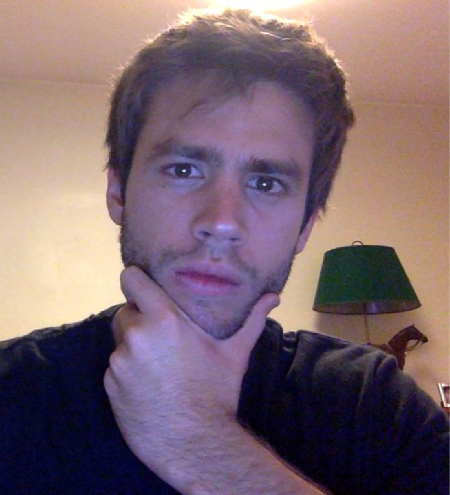
\includegraphics[width=3.5cm]{rvignolopic.png}\end{center}
\end{minipage}

\vspace{1cm plus \grande minus \grande}

% -=-=-=-=-=-=-=-=-=-=-=-=-=-=-=-=-=-=-=-=-=-=-=-=-=-=-=-=-=-=-=-=-=-=-=-=-=-=-=-=-=-=
\begin{secciontrescol}{Academic Formation}

\filatresentres{2014}{%
\emph{Nuclear Engineer}

Balseiro Institute, Cuyo National University \emph{\&} National Atomic Energy Commission. San Carlos de Bariloche.\\
Thesis: \href{http://ricabib.cab.cnea.gov.ar/467/}{\emph{Conceptual Design of a Compact Nuclear Research Reactor Core.}}\\
Advisors: PhD.~Eduardo Villarino and Eng.~Daniel Hergenreder.\\
INVAP S.E. Nuclear Engineering Department\\
GPA: 8.40/10.
}{\href{http://www.ib.edu.ar/index.php/english-version.html}{
\includegraphics[width=0.8cm]{logos/ib}}}{-0.6cm}

\filasep

\filadosentres{2011}{%
Completed the first two years of Aeronautical Engineering.\\
National Technological University, Haedo Regional Faculty.\\
GPA: 9.20/10.
}

\end{secciontrescol}


% -=-=-=-=-=-=-=-=-=-=-=-=-=-=-=-=-=-=-=-=-=-=-=-=-=-=-=-=-=-=-=-=-=-=-=-=-=-=-=-=-=-=
\begin{secciondoscol}{Languages}
 \filadosendos{Spanish}{Native language.}
 \filadosendos{English}{Speaks, reads and writes fluently.}
\end{secciondoscol}


% -=-=-=-=-=-=-=-=-=-=-=-=-=-=-=-=-=-=-=-=-=-=-=-=-=-=-=-=-=-=-=-=-=-=-=-=-=-=-=-=-=-=
\begin{secciondoscol}{Grants}

 \filadosendos{2011--2014}{Scholarship from the National Atomic Energy Commission (CNEA) to study Nuclear Engineering at the Balseiro Institute.\\}

\end{secciondoscol}

% -=-=-=-=-=-=-=-=-=-=-=-=-=-=-=-=-=-=-=-=-=-=-=-=-=-=-=-=-=-=-=-=-=-=-=-=-=-=-=-=-=-=
\begin{secciondoscol}{Programming languages}
 \filadosendos{C}{Advanced level.}
 \filadosendos{\CC}{Intermediate--advanced level.}
 \filadosendos{Python}{Intermediate level.}
 \filadosendos{Fortran}{Intermediate level.}
 \filadosendos{Scripting}{Intermediate level (including bash, AWK, sed, curl, etc).}
 \filadosendos{\LaTeX}{Advanced level.}
\end{secciondoscol}

% -=-=-=-=-=-=-=-=-=-=-=-=-=-=-=-=-=-=-=-=-=-=-=-=-=-=-=-=-=-=-=-=-=-=-=-=-=-=-=-=-=-=
\begin{secciontrescol}{Experience}

\filadosentres{\footnotesize 2017--current}{%
\azul{BESNA}, Buenos Aires\\
\emph{Engineering Consultant}
}

\filasep

\filadosentres{}{%
Detail engineering projects for Nuclear Power Plants.\\
Development of thermohydraulic calculation codes.\\
Specialist in calculations and analysis for Nuclear Power Reactors.
}

\filasep

\filadosentres{}{
\begin{tabular}{rp{\anchoparrafo}}
 Project & Numerical Simulation of the CAREM-25 Steam Generator\\
 Client  & National Atomic Energy Commission (CNEA)\\
 Period  & 2017--current \\
\end{tabular}}%
\nopagebreak%

\filadosentres{}{Development of the \emph{hhx} (\textbf{h}elical-coiled \textbf{h}eat e\textbf{X}changer) calculation code, capable of simulating two-phase flow in helical pipes and coupled with CFD tools (ANSYS CFX).}

\filasep

\filatresentres{\footnotesize 2014--current}{%
\azul{TECNA} Engineering Studies and Projects, Buenos Aires\\
\emph{S/Sr Nuclear Engineer}
}{\href{http://www.tecna.com/Home/tabid/40/language/en-US/Default.aspx}{
\includegraphics[width=0.8cm]{logos/tecna-solo}}}{-0.6cm}
\filadosentres{}{%
Detail engineering projects for Nuclear Power Plants.\\
Development of neutronic, thermohydraulic and control calculation codes.\\
Specialist in calculations and analysis for Nuclear Power Reactors.
}

\filasep

\filadosentres{}{
\begin{tabular}{rp{\anchoparrafo}}
 Project & CAREM-25 Balance of Plant\\
 Client  & National Atomic Energy Commission (CNEA)\\
 Period  & 2017--current \\
\end{tabular}}%
\nopagebreak%

\filadosentres{}{Intermediary between the supplier and the client in topics related to nuclear aspects.}
\filadosentres{}{Consultancy regarding operational modes of CAREM-25 reactor and their implications in the Balance of Plant (BOP).}

\filasep

\filadosentres{}{
\begin{tabular}{rp{\anchoparrafo}}
 Project & Specialized Nuclear Engineering Services for CNAI-II\\
 Client  & Nucleoeléctrica Argentina S.A.\\
 Period  & 2014--2016 \\
\end{tabular}}%
\nopagebreak%

\filadosentres{}{Development and implementation of the Method of Characteristics (MOC) for the resolution of the neutron transport equation in the milonga code (including \emph{ray tracing} algorithms).}

\filadosentres{}{Consultancy regarding neutron cell calculations for the obtention of condensed and homogenized macroscopic cross sections with DRAGON V5 lattice code in order to correctly model the doppler effect.}

\filadosentres{}{Nuclear engineering developments in neutron transport (cell) or diffusion (core) and thermohydraulics in PHWR.}

\filadosentres{}{Consultancy regarding spatial kinetics calculations coupled with plant and control codes.}

\filadosentres{}{Consultancy regarding the development of computational codes in order to reproduce coupled safety transients and update the Final Safety Analysis Report (FSAR) for Atucha~I Nuclear Power Plant.}

\filadosentres{}{Implementation of several updates for the neutron spatial kinetics programs (pcex and PCE2c).}

\filadosentres{}{Version control implementation (Git and Mercurial) for all the computational codes and technical documentation.}

\filadosentres{}{Implementation of DyPRA as a wasora plugin in order to increase the flexibility and traceability of executions (dypra2).}

\filadosentres{}{Engineering support for the Atucha~II Nuclear Power Plant start up. Doppler coefficient determination during commissioning stage.}

\filasep

\filatresentres{2013--2014}{%
\azul{INVAP S.E.} Nuclear Engineering Department, San Carlos de Bariloche \\
\emph{Undergraduate intern}
}{\href{http://www.invap.com.ar/en/}{
\includegraphics[width=0.8cm]{logos/invap}}}{-0.6cm}

% \nopagebreak
 \filadosentres{}{ 
\begin{tabular}{rp{\anchoparrafo}}
 Project & Internship. \\ 
 Period & 2013--2014 \\
 Assignment &

 Nuclear engineering thesis: \href{http://ricabib.cab.cnea.gov.ar/467/}{\emph{Conceptual Design of a Compact Nuclear Research Reactor Core.}} \\
\end{tabular}
}

\filasep
 
\filatresentres{2011--2014}{%
\azul{CNEA} National Atomic Energy Commission, Bariloche Atomic Centre\\
\emph{Scholarship -- Student}
}{\href{http://www.cnea.gov.ar}{
\includegraphics[width=0.8cm]{logos/cnea}}}{-0.6cm}

\filadosentres{}{Studies carried out at the Balseiro Institute under the scholarship granted by the National Atomic Energy Commission to obtain the Nuclear Engineer title.}

\end{secciontrescol}


% -=-=-=-=-=-=-=-=-=-=-=-=-=-=-=-=-=-=-=-=-=-=-=-=-=-=-=-=-=-=-=-=-=-=-=-=-=-=-=-=-=-=
\begin{secciontrescol}{Refereed Publications}

\paper{2016}{Vignolo, R.}{Solving the neutron transport equation by the method of characteristics in milonga neutron code}{III Annual Meeting of the Argentine Reactor Calculation and Analysis Group\\XLIII Annual Meeting of the Argentine Association of Nuclear Technology}{https://bitbucket.org/rvignolo/aatn-2016-moc-milonga}{aatn-2016-3}

\paper{2016}{Vignolo, R., Schivo, M.}{Doppler coefficient: Comparisons between measurements and kinetic calculations for the Atucha~II Nuclear Power Plant}{XLIII Annual Meeting of the Argentine Association of Nuclear Technology}{https://bitbucket.org/rvignolo/aatn-2016-appl-multi-xs}{aatn-2016-2}

\paper{2016}{Vignolo, R., Giuntoli, G., Khatchikian, F.}{Development of multiple parameters cross sections tables in DRAGON V5 for the Atucha~II Nuclear Power Plant}{XLIII Annual Meeting of the Argentine Association of Nuclear Technology}{https://bitbucket.org/rvignolo/aatn-2016-xs-multitabla}{aatn-2016-1}

\paper{2015}{Vignolo, R., San Sebastián, G.}{Implementation of routines for the extraction and insertion of fuel elements in DyPRA's suite}{XLII Annual Meeting of the Argentine Association of Nuclear Technology}{https://bitbucket.org/rvignolo/aatn-2015-ext-ins-eecc}{aatn-2015}

\paper{2014}{Vignolo, R., Villarino, E.}{Conceptual Design of a Compact Nuclear Reactor Core}{XVI meeting of the International Group On Research Reactors}{http://www.igorr.com/scripts/home/publigen/content/templates/Show.asp?P=1000&L=EN}{igorr-2014}

\paper{2014}{Vignolo, R., Villarino, E.}{Conceptual Design of a Compact Nuclear Research Reactor Core}{Graduate thesis at Balseiro Institute.}{http://ricabib.cab.cnea.gov.ar/467/}{tesis-ib}

\end{secciontrescol}


% -=-=-=-=-=-=-=-=-=-=-=-=-=-=-=-=-=-=-=-=-=-=-=-=-=-=-=-=-=-=-=-=-=-=-=-=-=-=-=-=-=-=
\begin{secciontrescol}{Technical Reports}
\report{2016}{R. Vignolo, G. Giuntoli, TECNA~S.A.}{Doppler coefficient: Comparisons between measurements and kinetic calculations of Atucha~II Nuclear Power Plant}{ 10527-N-IT16-318 }{}{}

\report{2016}{R. Vignolo, G. Giuntoli, TECNA~S.A.}{Atucha~II DRAGON fuel cell: calculating multi-dependent cross sections}{ 10527-N-IT16-317 }{}{}

\report{2015}{J.P. Gómez Omil, A. Tarazaga, R. Vignolo, G. Theler , TECNA~S.A.}{Cálculo de coeficientes para las ecuaciones puntuales de iodo-135 y xenón-135 a partir de distribuciones espaciales de secciones eficaces y propiedades nucleares}{ 10527-N-IT15-309 }{}{}

\report{2015}{R. Vignolo, J. P. Gómez Omil, A. Tarazaga, TECNA~S.A.}{Cálculo de coeficientes de reactividad y curvas de reactividad de bancos de barras de la Central Nuclear Atucha~I}{ 10527-N-IT15-308 }{}{}

\report{2015}{R. Vignolo, J. P. Gómez Omil, TECNA~S.A.}{Determinación y análisis de la reactividad insertada por el boro proveniente del segundo sistema de extinción de la Central Nuclear Atucha~I para dos y tres lanzas}{ 10527-N-IT15-307 }{}{}

\report{2015}{A. Tarazaga, G. Theler, R. Vignolo, TECNA~S.A.}{Modelado en PCEx de la nube de boro correspondiente al Segundo Sistema de Extinción de la Central Nuclear Atucha~I}{ 10527-N-IT15-306 }{}{}

\report{2015}{R. Vignolo, G. Theler, TECNA~S.A.}{Estimaci\'on del coeficiente de reactividad por temperatura del combustible con n\'ucleo  en equilibrio al 100 por ciento de potencia}{ 10527-N-IT15-109 }{}{}

\report{2014}{R. Vignolo, G. Theler, TECNA~S.A.}{Estimaci\'on del coeficiente de reactividad por temperatura del combustible con n\'ucleo  en equilibrio al 90 por ciento de potencia}{ 10527-N-IT15-108 }{}{}

\report{2014}{R. Vignolo, TECNA~S.A.}{Implementación de rutinas para la extracción e inserción de elementos combustibles en PCE2c dentro de la plataforma DyPRA}{ 10527-N-IT15-202 }{}{}


\end{secciontrescol}

% -=-=-=-=-=-=-=-=-=-=-=-=-=-=-=-=-=-=-=-=-=-=-=-=-=-=-=-=-=-=-=-=-=-=-=-=-=-=-=-=-=-=
\begin{secciontrescol}{Conference presentations}

\congreso{2016}{III Annual Meeting of the Argentine Reactor Calculation and Analysis Group, Buenos Aires}%
%
\presentacion{Vignolo, R.}{Hands on DRAGON: learning how to use DRAGON V5 for cross section production}{https://bitbucket.org/rvignolo/taller-dragon-garcar-2016}{garcar-2016-2}

\presentacion{Vignolo, R.}{Solving the neutron transport equation by the method of characteristics in milonga neutron code}{https://bitbucket.org/rvignolo/aatn-2016-moc-milonga-presentacion}{garcar-2016-1}

\congreso{2016}{XLIII Annual Meeting of the Argentine Association of Nuclear Technology, Buenos Aires}%
%
\presentacion{Vignolo, R., Giuntoli, G., Khatchikian, F.}{Development of multiple parameters cross sections tables in DRAGON V5 for Atucha~II Nuclear Power Plant}{https://bitbucket.org/rvignolo/aatn-2016-xs-multitabla-presentacion}{aatn-2016-1-pres}
%
\presentacion{Vignolo, R., Schivo, M.}{Doppler coefficient: Comparisons between measurements and kinetic calculations for the Atucha~II Nuclear Power Plant}{https://bitbucket.org/rvignolo/aatn-2016-appl-multi-xs-presentacion}{aatn-2016-2-pres}
%
\presentacion{Vignolo, R.}{Solving the neutron transport equation by the method of characteristics in milonga neutron code}{https://bitbucket.org/rvignolo/aatn-2016-moc-milonga-presentacion}{aatn-2016-3-pres}

\congreso{2015}{XLII Annual Meeting of the Argentine Association of Nuclear Technology, Buenos Aires}%
%
\presentacion{Vignolo, R., San Sebastián, G.}{Implementation of routines for the extraction and insertion of fuel elements in DyPRA's suite}{https://bitbucket.org/seamplex/wasora}{wasora}

\end{secciontrescol}


% -=-=-=-=-=-=-=-=-=-=-=-=-=-=-=-=-=-=-=-=-=-=-=-=-=-=-=-=-=-=-=-=-=-=-=-=-=-=-=-=-=-=
\begin{secciontrescol}{Freen and open software}

\software{wasora}{Wasora is a convenient high-level interface to perform mathematical computations. It also provides a framework which other particular computational codes can use. It is a free computational tool designed to aid a cognizant expert to analyze complex systems by solving mathematical problems by means of a high-level plain-text}{https://bitbucket.org/seamplex/wasora}

\software{milonga}{Milonga is a free core-level neutronic code that solves the steady-state multigroup neutron transport equation (using the diffusion approximation, discrete ordinates $S_N$ method or the method of characteristics) over unstructured grids (although simple structured grids can also be used) using either a finite-volumes or a finite-elements discretization scheme.}{https://bitbucket.org/rvignolo/milonga}

\end{secciontrescol}


% -=-=-=-=-=-=-=-=-=-=-=-=-=-=-=-=-=-=-=-=-=-=-=-=-=-=-=-=-=-=-=-=-=-=-=-=-=-=-=-=-=-=
\begin{secciondoscol}{Advice}
 \filadosendos{2016}{Vocal Press and Communication for the Argentine Youth Nuclear Generation (AYNG).\\}
\end{secciondoscol}

% \pagebreak


\vspace{\fill}
\hspace{0.6\linewidth}
\begin{minipage}{0.35\linewidth}
 \begin{center}
 Ramiro Vignolo\\
% version tracking
\immediate\write18{./date.sh > date.tex }
\immediate\write18{./hash.sh > hash.tex }

\makeatletter
\ifcase\pdf@shellescape
  \today\or
  \input{date}\or
  \today\fi

\scriptsize{\texttt{
\ifcase\pdf@shellescape
  unknown revision hash, re-compile with '--shell-escape'\or
  \input{hash}\or
  unknown revision hash, re-compile with '--shell-escape'\fi
}}
\makeatother
 
 \end{center}
\end{minipage}


\end{document}
